\begin{figure}[h!]
    \centering
    \caption{Changes in log rents and log total wages under counterfactual
             minimum wage policies, Chicago-Naperville-Elgin CBSA}
    \label{fig:map_chicago_cf_rents_wages}

    \begin{minipage}{.95\textwidth} \centering
        Panel A: Increase in federal MW from \$7.25 to \$9
        \vspace{1.5mm}
    \end{minipage}
    
    \begin{subfigure}{.4\textwidth}  \centering
        \caption*{Changes in log rents}
        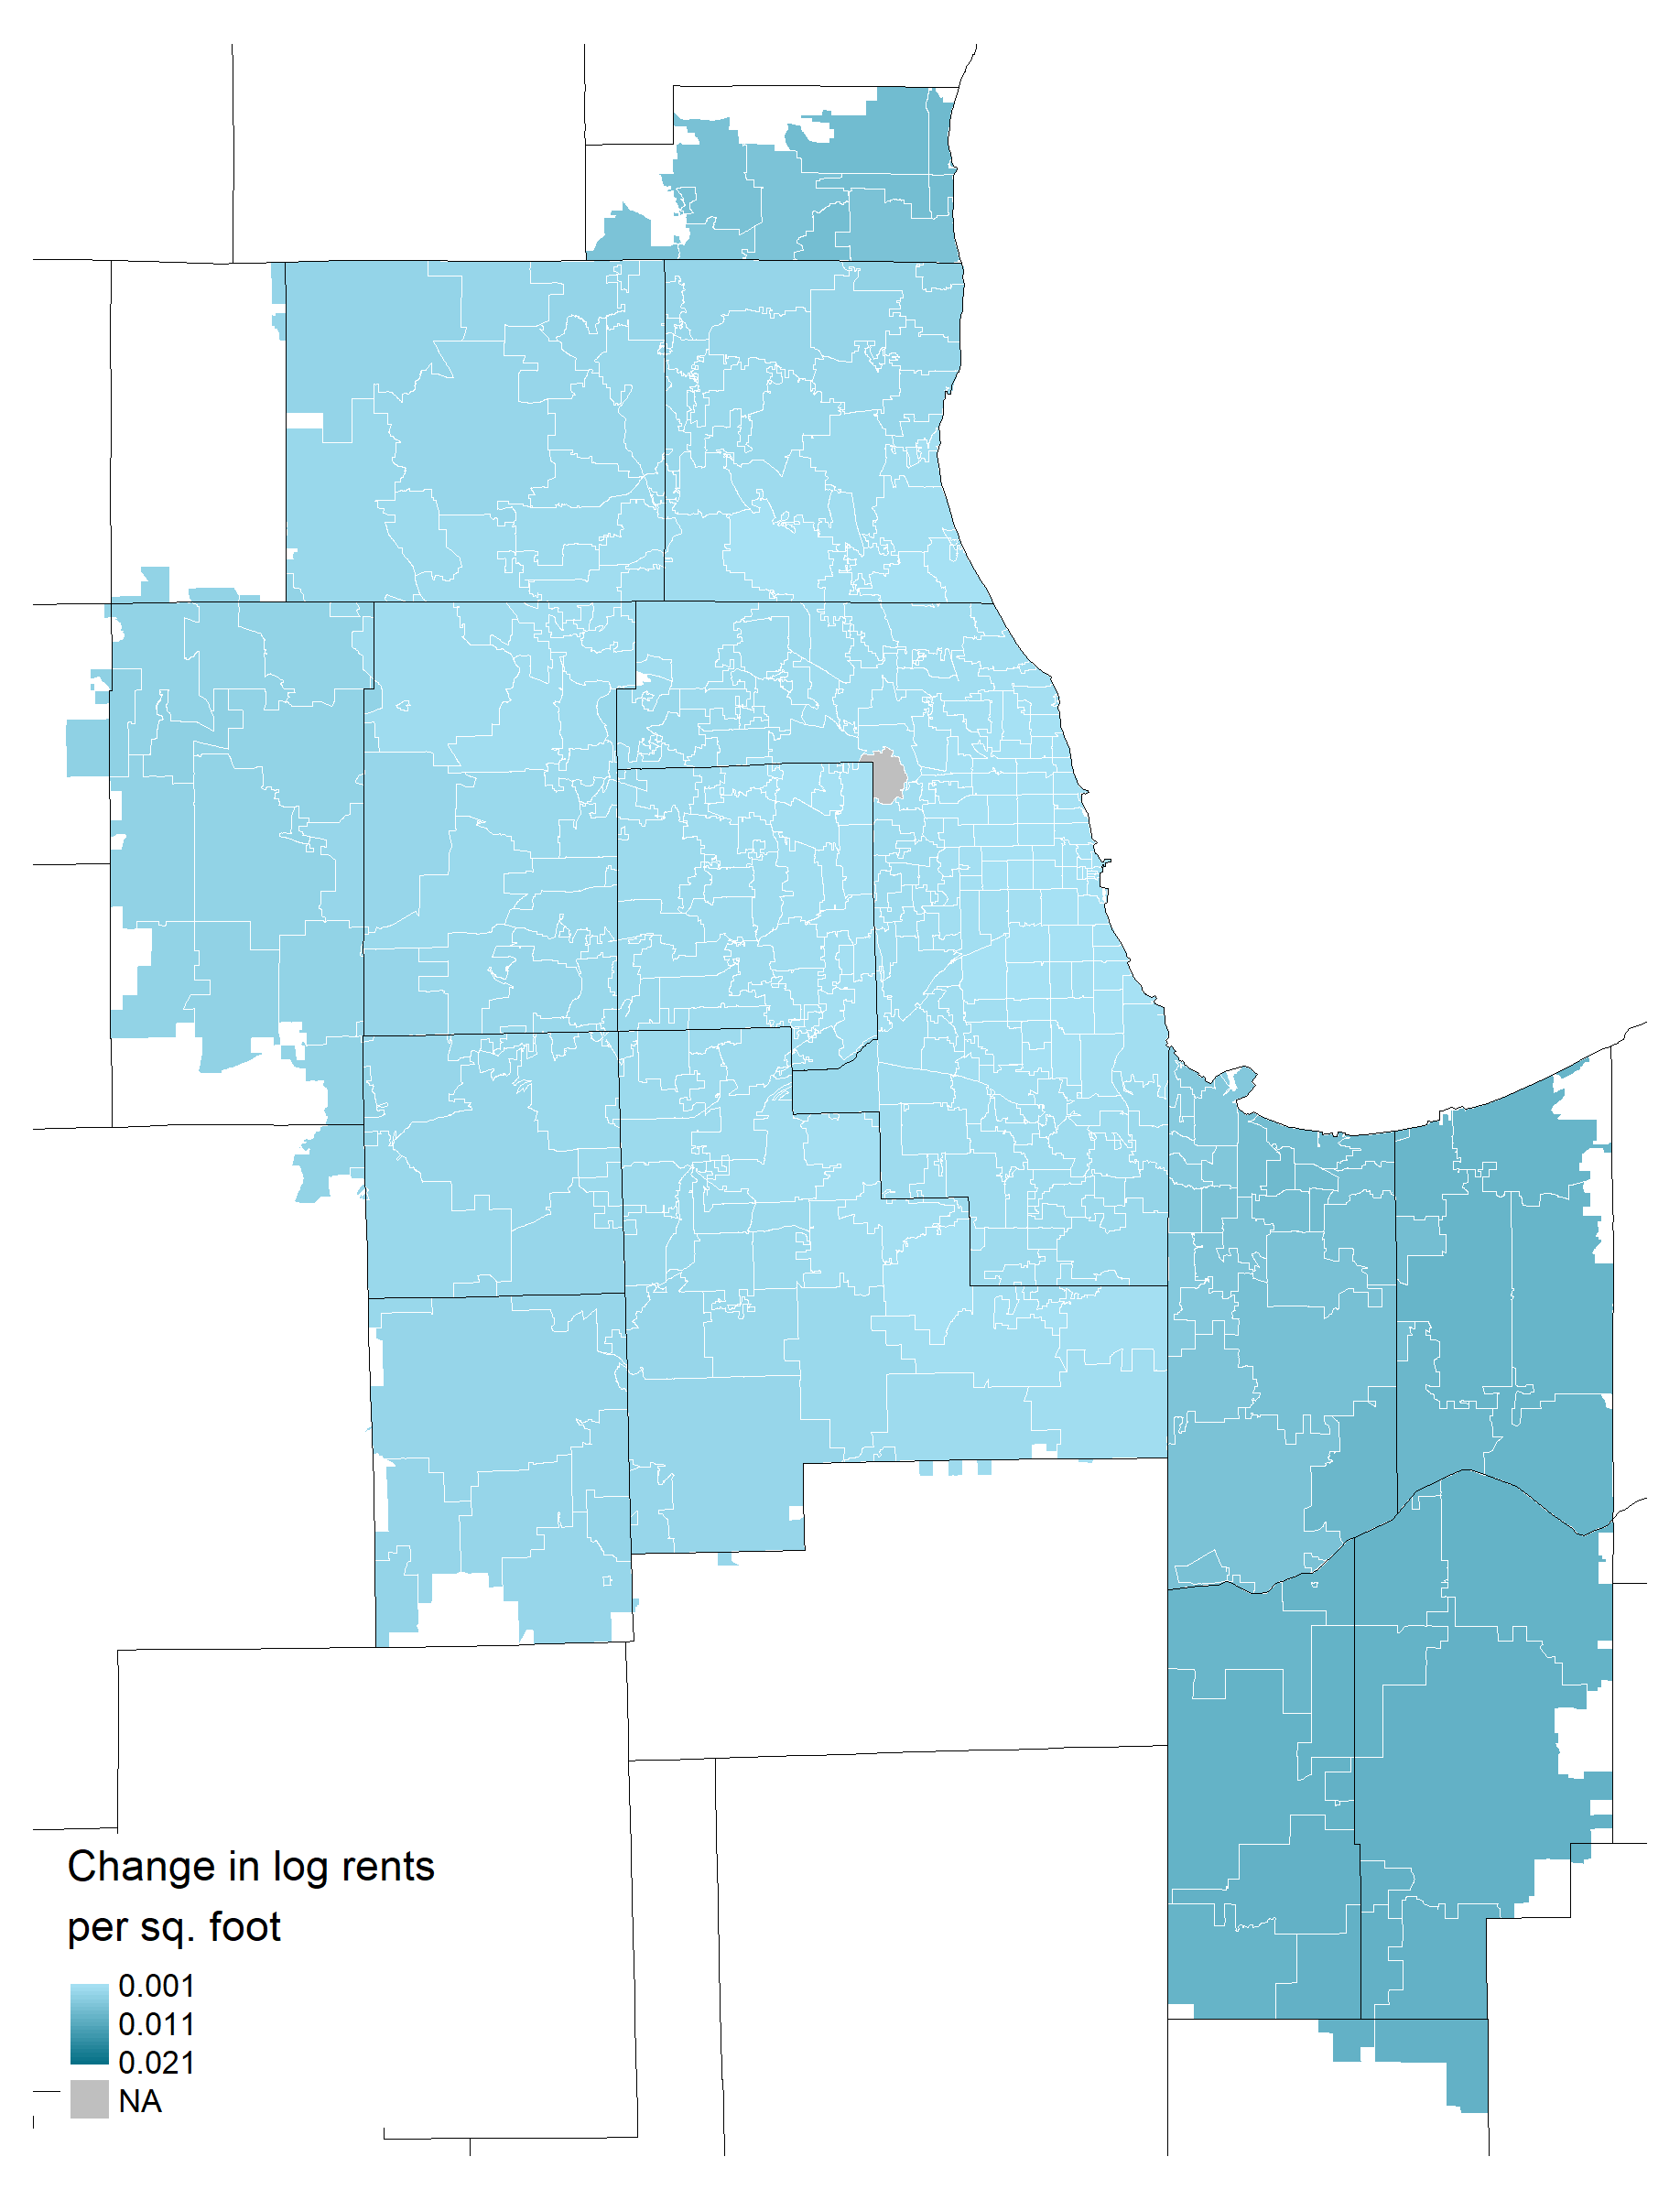
\includegraphics[width = 1\textwidth]
            {counterfactuals/output/chicago_d_ln_rents_fed_9usd_png}
    \end{subfigure}%
    $\quad\quad\quad\quad$%
    \begin{subfigure}{.4\textwidth}  \centering
        \caption*{Changes in log total wages}
        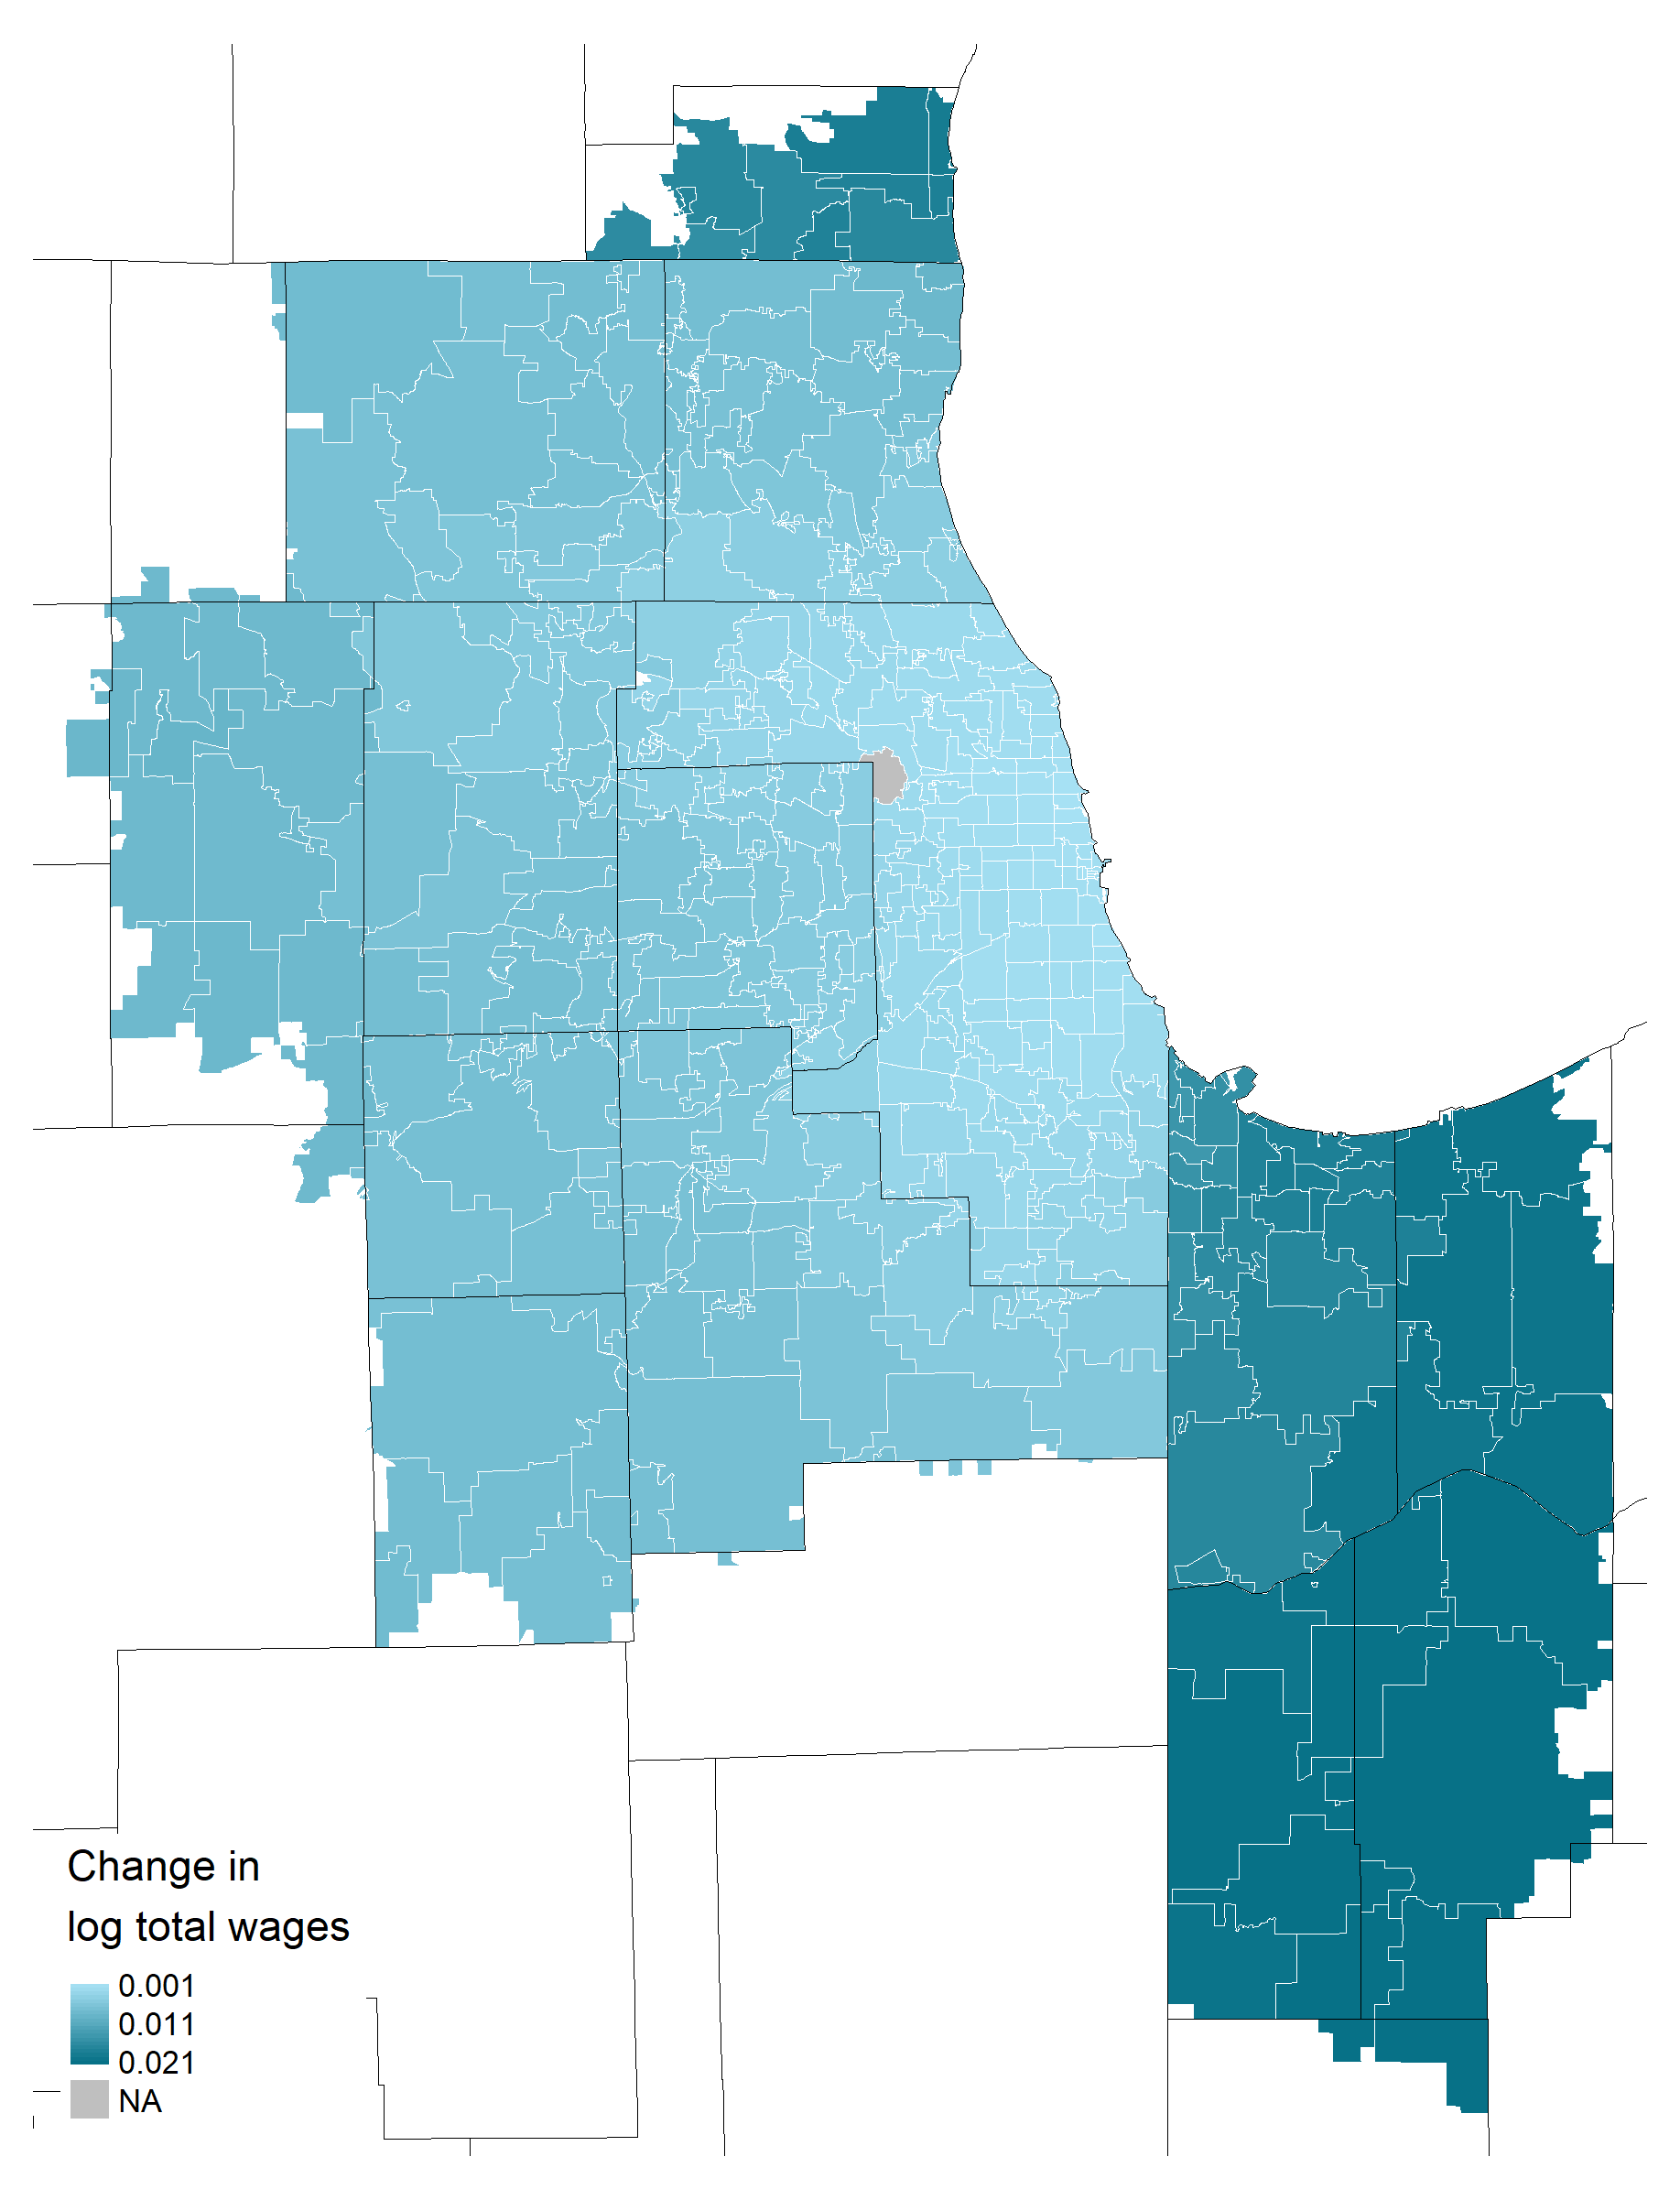
\includegraphics[width = 1\textwidth]
            {counterfactuals/output/chicago_d_ln_wagebill_fed_9usd_png}
    \end{subfigure}

    \begin{minipage}{.95\textwidth} \centering
        \vspace{2mm}
        Panel B: Increase in Chicago MW from \$13 to \$14
        \vspace{1.5mm}
    \end{minipage}
    
    \begin{subfigure}{.4\textwidth}  \centering
        \caption*{Changes in log rents}
        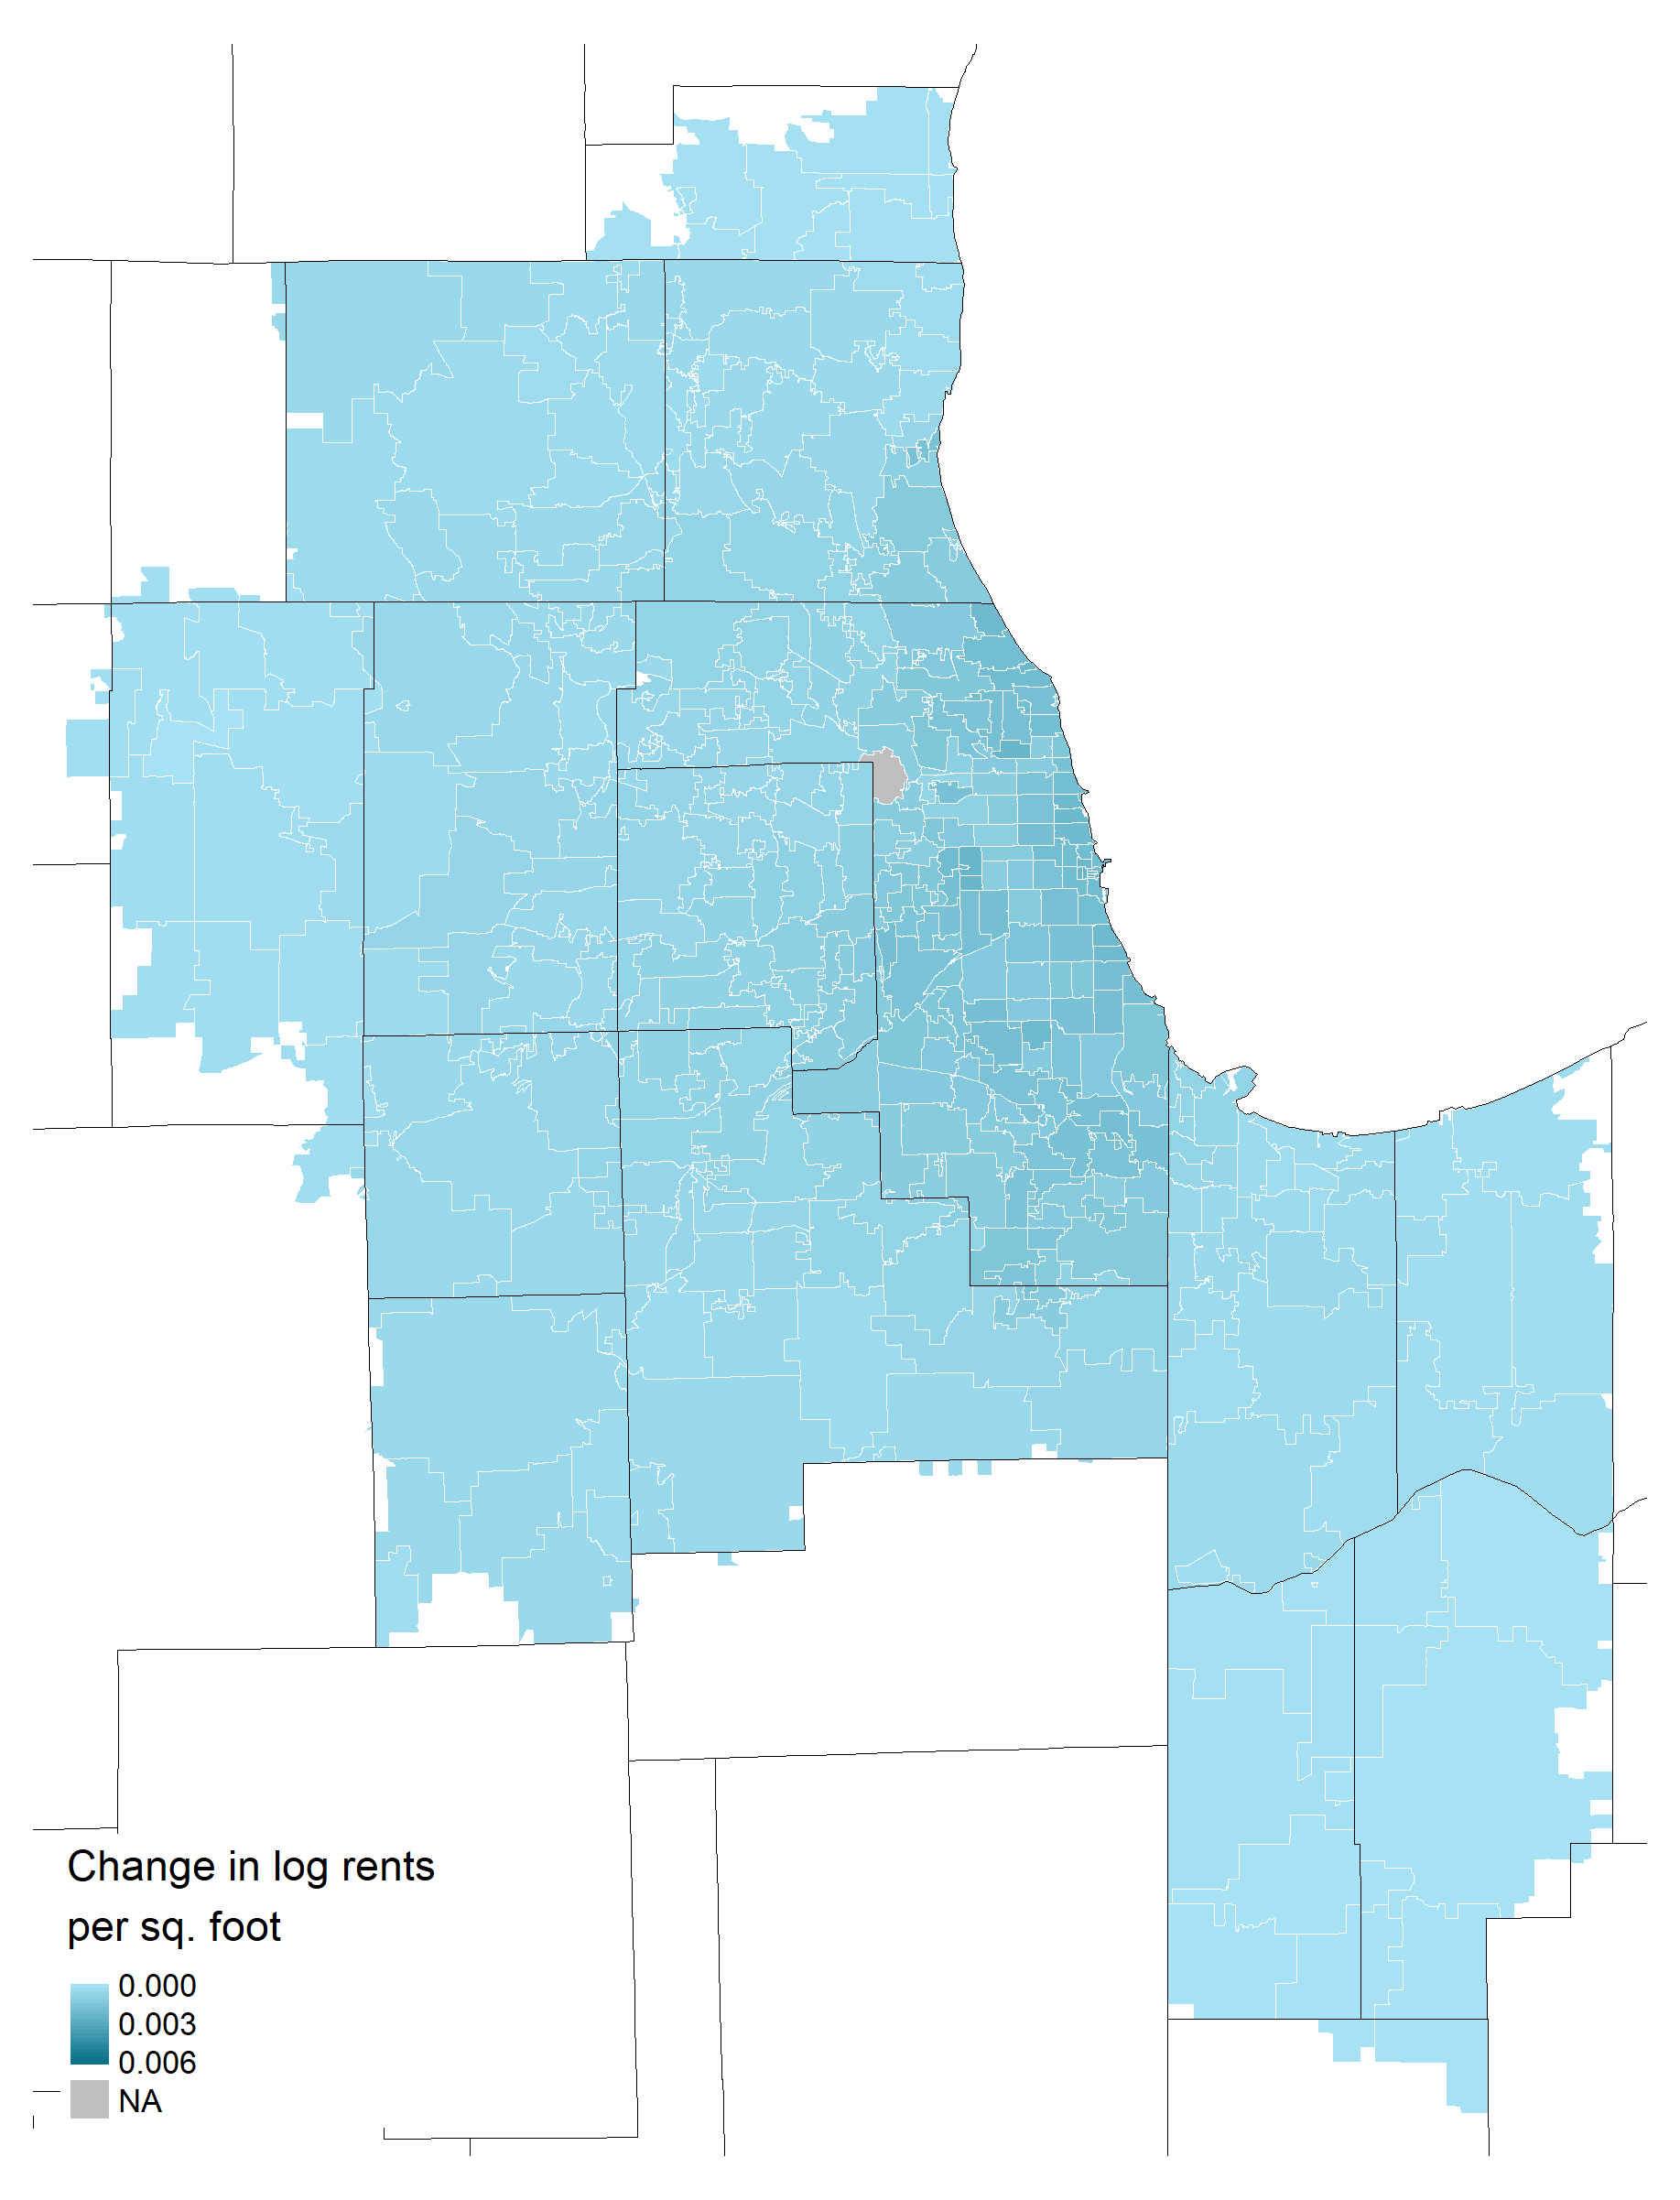
\includegraphics[width = 1\textwidth]
            {counterfactuals/output/chicago_d_ln_rents_chi14_png}
    \end{subfigure}%
    $\quad\quad\quad\quad$%
    \begin{subfigure}{.4\textwidth}  \centering
        \caption*{Changes in log total wages}
        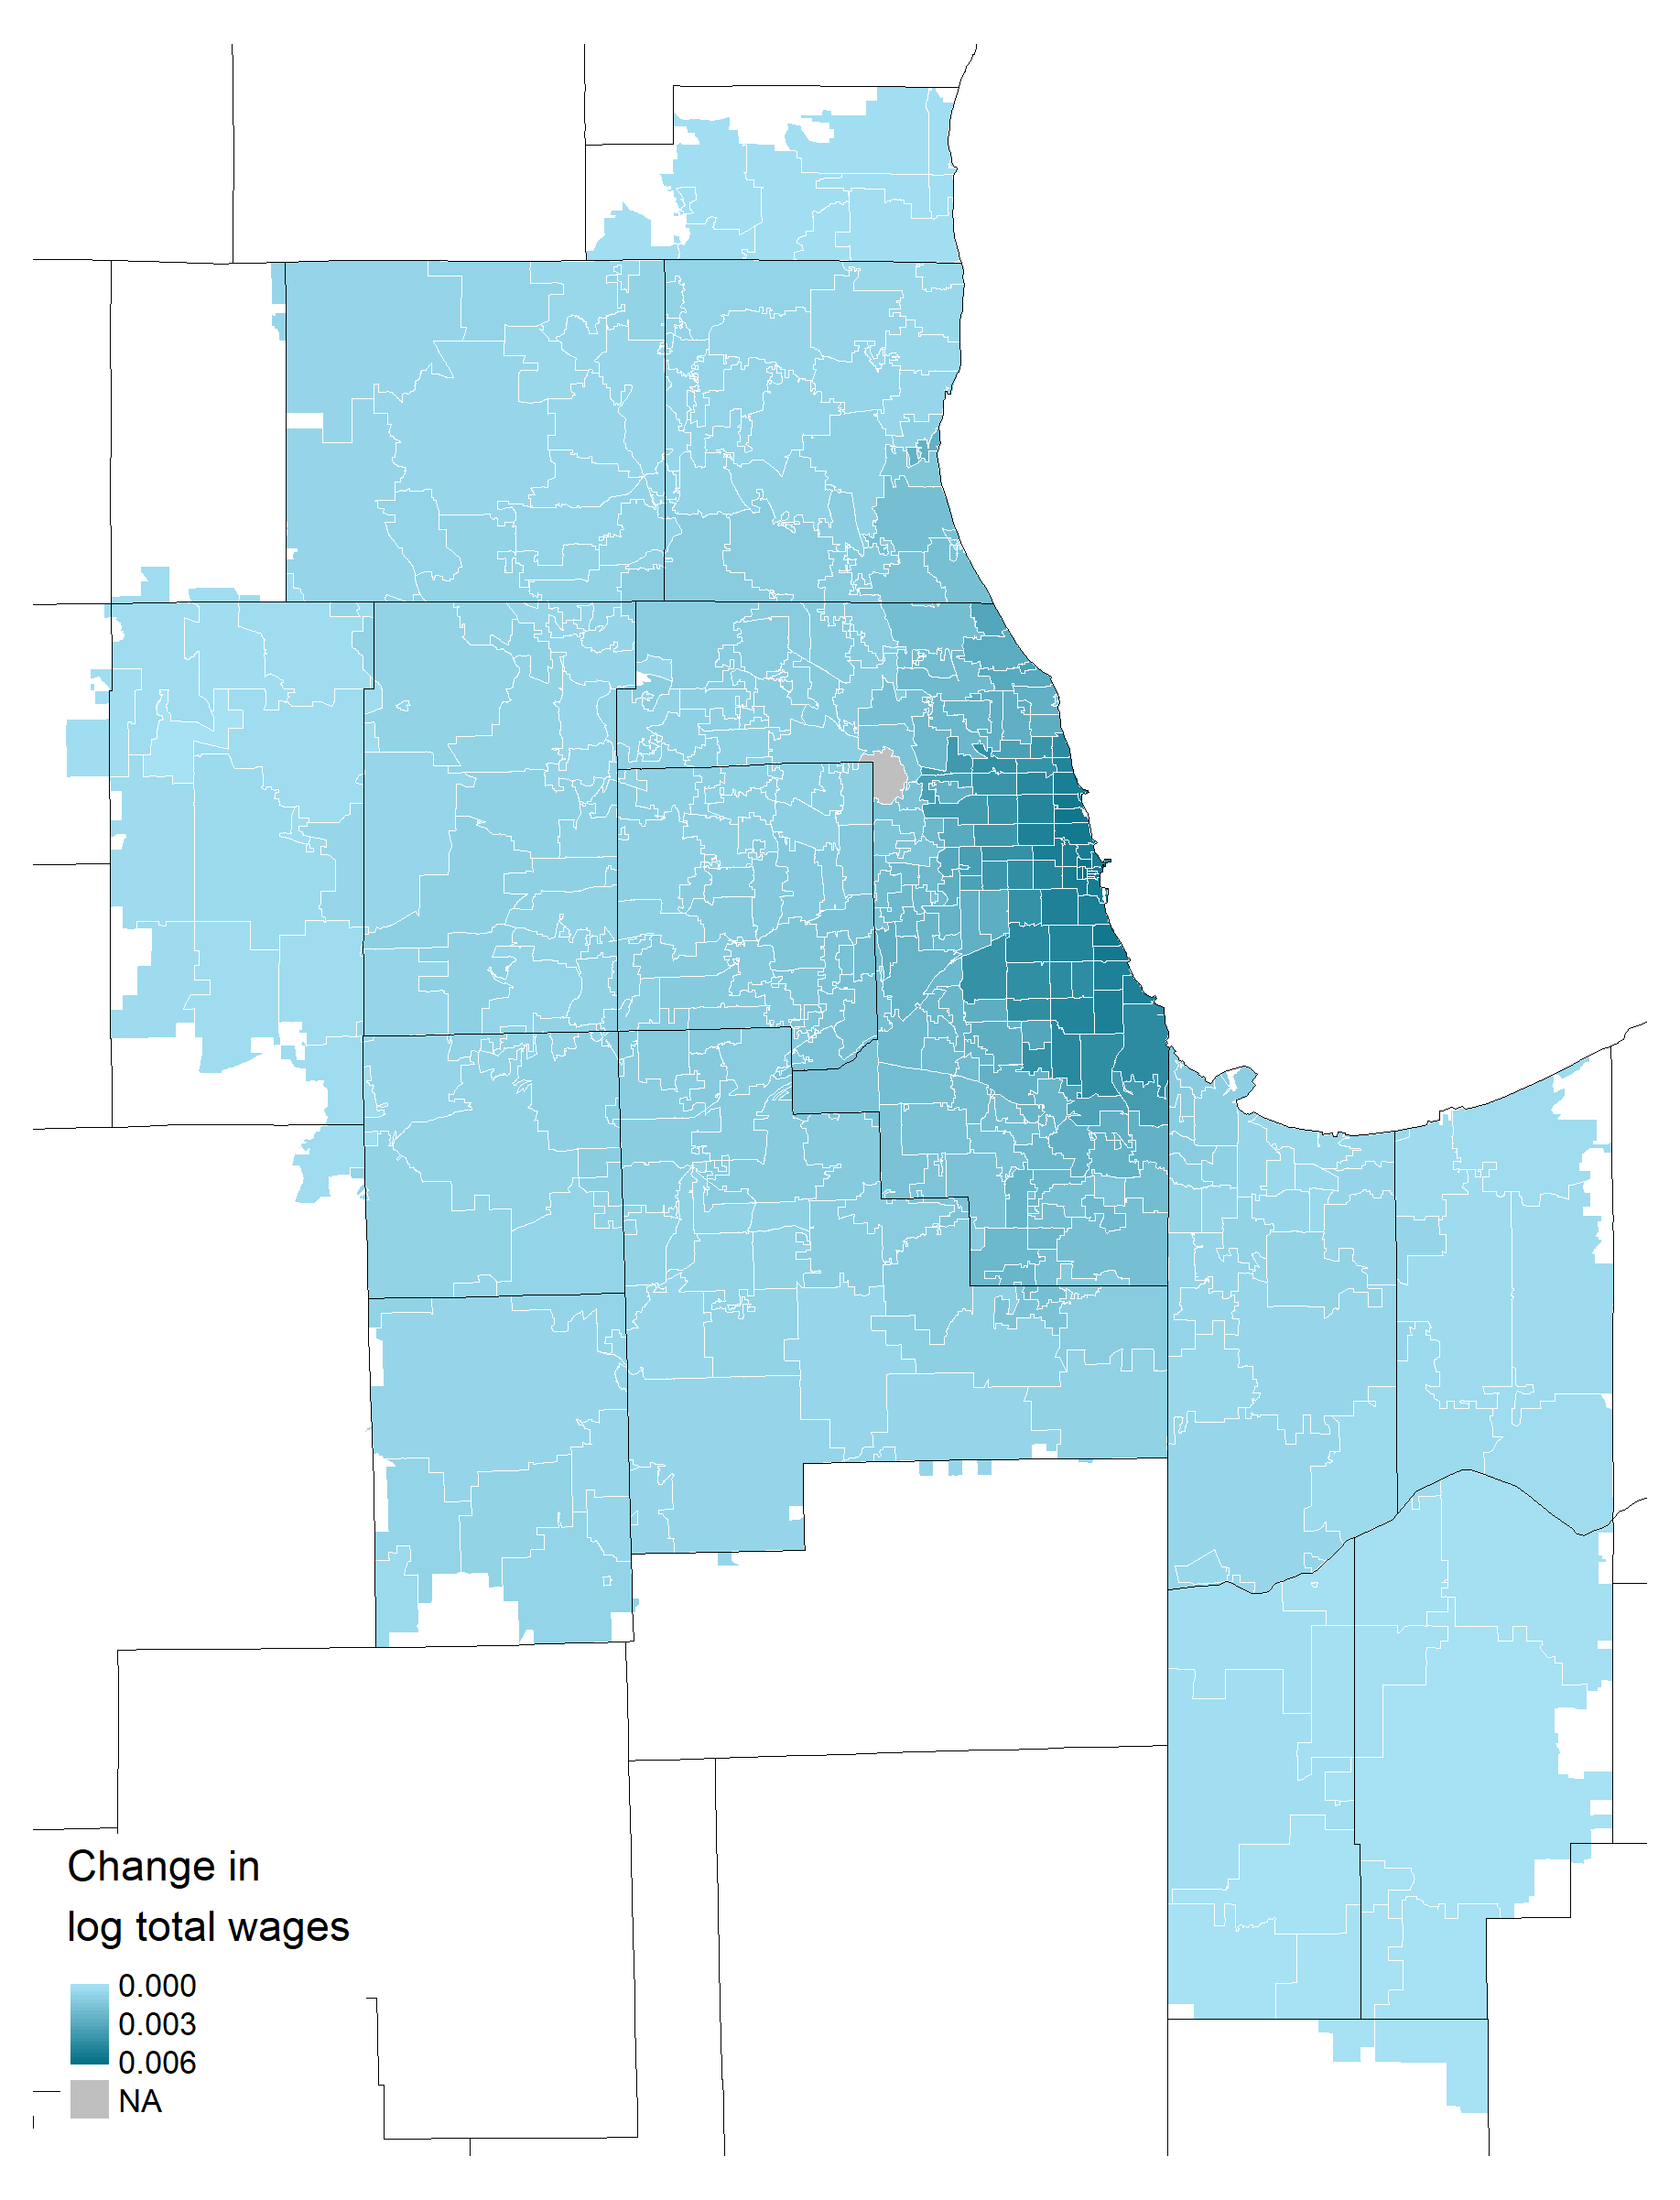
\includegraphics[width = 1\textwidth]
            {counterfactuals/output/chicago_d_ln_wagebill_chi14_png}
    \end{subfigure}

    \begin{minipage}{.95\textwidth} \footnotesize
        \vspace{2.5mm}
        Notes: 
        Data are from the MW panel described in section \ref{sec:data_mw_panel} 
        and from LODES.
        The figures map the estimated changes in log total rents per square foot
        and log total wage income under different counterfactual MW policies 
        in the Chicago-Naperville-Elgin CBSA.
        Panel A is based on a counterfactual increase to \$9 in the 
        federal MW in January 2020, holding constant other MW policies in their 
        December 2019 levels.
        Panel B is based on a counterfactual increase from \$13 to \$14 in the 
        Chicago City MW, also holding constant other MW policies.
        The color scale has been standardized within each panel.
        To estimate the changes we follow the procedure described in Section 
        \ref{sec:counterfactual} assuming the following parameter values: 
        $\beta = \betaCf$, $\gamma = \gammaCf$, and $\varepsilon = \epsilonCf$.
    \end{minipage}
\end{figure}
